%%% File-Information {{{
%%% Filename: template.tex
%%% Purpose: lab report, technical report, project report
%%% Time-stamp: <2023-10-16 11:16 xx>
%%% Authors: Maximilian Gerner
%%%          
%%% History:
%%%   20231016 (mg) initial version
%%%
%%% Notes:
%%%
%%%
%%%
%%% }}}
%%%%%%%%%%%%%%%%%%%%%%%%%%%%%%%%%%%%%%%%%%%%%%%%%%%%%%%%%%%%%%%%%%%%%%%%%%%%%%%%
%%% main document {{{

\documentclass[
a4paper,     %% defines the paper size: a4paper (default), a5paper, letterpaper, ...
% landscape,   %% sets the orientation to landscape
% twoside,     %% changes to a two-page-layout (alternatively: oneside)
% twocolumn,   %% changes to a two-column-layout
 headsepline, %% add a horizontal line below the column title
% footsepline, %% add a horizontal line above the page footer
% titlepage,   %% only the titlepage (using titlepage-environment) appears on the first page (alternatively: notitlepage)
 halfparskip,     %% insert an empty line between two paragraphs (alternatively: halfparskip, ...)
% leqno,       %% equation numbers left (instead of right)
 fleqn,       %% equation left-justified (instead of centered)
% tablecaptionabove, %% captions of tables are above the tables (alternatively: tablecaptionbelow)
% draft,       %% produce only a draft version (mark lines that need manual edition and don't show graphics)
% 10pt         %% set default font size to 10 point
% 11pt         %% set default font size to 11 point
12pt         %% set default font size to 12 point
]{scrartcl}  %% article, see KOMA documentation (scrguide.dvi)


%%%%%%%%%%%%%%%%%%%%%%%%%%%%%%%%%%%%%%%%%%%%%%%%%%%%%%%%%%%%%%%%%%%%%%%%%%%%%%%%
%%%
%%% define the titlepage
%%%
%%%
%%% Notes: substitute variables are used because \maketitle clears 
%%% \title, \author etc.
%%%

\def\getsubject{Bericht}   
\subject{\getsubject}   %% subject which appears above titlehead
% \titlehead{} %% special heading for the titlepage


%%% title
\def\gettitle{Untersuchung einer Antriebswelle}
\title{\gettitle}


%%% author(s) use \and for more than one author (search for workaround with the warnings thrown by hyperrefsetup
\def\getauthor{Maximilian Gerner}
\author{\getauthor}

%%% date
\def\getdate{Graz, Wintersemester 2023}
\date{\getdate}

% \publishers{}

% \thanks{} %% use it instead of footnotes (only on titlepage)

% \dedication{} %% generates a dedication-page after titlepage


%%%%%%%%%%%%%%%%%%%%%%%%%%%%%%%%%%%%%%%%%%%%%%%%%%%%%%%%%%%%%%%%%%%%%%%%%%%%%%%%
%%%
%%% packages
%%%

%%%
%%% encoding and language set
%%%

%%% ngerman: language set to new-german
\usepackage{ngerman}

%%% babel: language set (can cause some conflicts with package ngerman)
%%%        use it only for multi-language documents or non-german ones
%\usepackage[ngerman]{babel}

%%% inputenc: coding of german special characters
\usepackage[utf8]{inputenc}

%%% for Linux:
% \usepackage[latin1]{inputenc}

%%% fontenc, ae, aecompl: coding of characters in PDF documents
\usepackage[T1]{fontenc}
\usepackage{ae,aecompl}

%%%
%%% technical packages
%%%

%%% amsmath, amssymb, amstext: support for mathematics
\usepackage{amsmath,amssymb,amstext}

%%% psfrag: replace PostScript fonts
%\usepackage{psfrag}

%%% listings: include programming code
%\usepackage{listings}

%%% units: technical units
\usepackage{units}

%%%
%%% layout
%%%

%%% scrlayer-scrpage: KOMA heading and footer
%%% Note: if you don't use this package, please remove 
%%%       \pagestyle{scrheadings} and corresponding settings
%%%       below too.
\usepackage{scrlayer-scrpage}






%%%
%%% PDF
%%%

\newif\ifpdf
  \ifx\pdfoutput\undefined
     \pdffalse
  \else
     \pdfoutput=1
     \pdftrue
  \fi

%%% Should be LAST usepackage-call!
%%% For docu on that, see reference on package ``hyperref''
\Ifpdfoutput{%   (definitions for using pdflatex instead of latex)

  %%% graphicx: support for graphics
  \usepackage[pdftex]{graphicx}

  \pdfcompresslevel=9

  %%% hyperref (hyperlinks in PDF): for more options or more detailed
  %%%          explanations, see the documentation of the hyperref-package
  \usepackage[%
    %%% general options
    %pdftex=true,      %% sets up hyperref for use with the pdftex program
    %plainpages=false, %% set it to false, if pdflatex complains: ``destination with same identifier already exists''
    %
    %%% extension options
    backref=page,      %% if page, adds a backlink text to the end of each item in the bibliography that points to the page where the source is cited
    pagebackref=false, %% if true, creates backward references as a list of page numbers in the bibliography
    colorlinks=true,   %% turn on colored links (true is better for on-screen reading, false is better for printout versions)
    %
    %%% PDF-specific display options
    bookmarks=true,          %% if true, generate PDF bookmarks (requires two passes of pdflatex)
    bookmarksopen=false,     %% if true, show all PDF bookmarks expanded
    bookmarksnumbered=false, %% if true, add the section numbers to the bookmarks
    %pdfstartpage={1},        %% determines, on which page the PDF file is opened
    pdfpagemode=UseNone         %% None, UseOutlines (=show bookmarks), UseThumbs (show thumbnails), FullScreen
  ]{hyperref}


  %%% provide all graphics (also) in this format, so you don't have
  %%% to add the file extensions to the \includegraphics-command
  %%% and/or you don't have to distinguish between generating
  %%% dvi/ps (through latex) and pdf (through pdflatex)
  \DeclareGraphicsExtensions{.pdf}

}{%else   (definitions for using latex instead of pdflatex)

  \usepackage[dvips]{graphicx}

  \DeclareGraphicsExtensions{.eps}

  \usepackage[%
    dvips,           %% sets up hyperref for use with the dvips driver
    colorlinks=false %% better for printout version; almost every hyperref-extension is eliminated by using dvips
  ]{hyperref}

}


%%% sets the PDF-Informations options
%%% (see fields in Acrobat Reader: ``File -> Document properties -> Summary'')
%%% Note: this method is better than as options of the hyperref-package (options are expanded correctly)
\hypersetup{
  pdftitle={\gettitle}, %%
  pdfauthor={\getauthor}, %%
  pdfsubject={\getsubject}, %%
  pdfcreator={Accomplished with LaTeX2e and pdfLaTeX with hyperref-package.}, %% 
  pdfproducer={}, %%
  pdfkeywords={} %%
}


%%%%%%%%%%%%%%%%%%%%%%%%%%%%%%%%%%%%%%%%%%%%%%%%%%%%%%%%%%%%%%%%%%%%%%%%%%%%%%%%
%%%
%%% user defined commands
%%%

%%% \mygraphics{}{}{}
%% usage:   \mygraphics{width}{filename_without_extension}{caption}
%% example: \mygraphics{0.7\textwidth}{rolling_grandma}{This is my grandmother on inlinescates}
%% requires: package graphicx
%% provides: including centered pictures/graphics with a boldfaced caption below
%% 
\newcommand{\mygraphics}[3]{
  \begin{center}
    \includegraphics[width=#1, keepaspectratio=true]{#2} \\
    \textbf{#3}
  \end{center}
}


%%%%%%%%%%%%%%%%%%%%%%%%%%%%%%%%%%%%%%%%%%%%%%%%%%%%%%%%%%%%%%%%%%%%%%%%%%%%%%%%
%%%
%%% set heading and footer
%%%

%%% scrheadings default: 
%%%      footer - middle: page number
\pagestyle{scrheadings}

%%% user specific
%%% usage:
%%% \position[heading/footer for the titlepage]{heading/footer for the rest of the document}

%%% heading - left
% \ihead[]{}

%%% heading - center
% \chead[]{}

%%% heading - right
 \ohead[]{\gettitle}

%%% footer - left
% \ifoot[]{}

%%% footer - center
% \cfoot[]{}

%%% footer - right
% \ofoot[]{}



%%%%%%%%%%%%%%%%%%%%%%%%%%%%%%%%%%%%%%%%%%%%%%%%%%%%%%%%%%%%%%%%%%%%%%%%%%%%%%%%
%%%
%%% begin document
%%%

\begin{document}




 \pagenumbering{roman} %% small roman page numbers

%%% include the title
% \thispagestyle{empty}  %% no header/footer (only) on this page
 \maketitle



%%% start a new page and display the table of contents
% \newpage
 \tableofcontents

%%% start a new page and display the list of figures
% \newpage
 \listoffigures

%%% start a new page and display the list of tables
% \newpage
 \listoftables

%%% display the main document on a new page 
 \newpage

 \pagenumbering{arabic} %% normal page numbers (include it, if roman was used above)

%%%%%%%%%%%%%%%%%%%%%%%%%%%%%%%%%%%%%%%%%%%%%%%%%%%%%%%%%%%%%%%%%%%%%%%%%%%%%%%%
%%%
%%% begin main document
%%% structure: \section \subsection \subsubsection \paragraph \subparagraph
%%%



\section{Einleitung}
\label{sec:einleitung}

Ziel dieser Arbeit ist es weniger, eine Antriebswelle auf ihre Belastung durchzurechnen, als vielmehr ein Beispiel zu bringen, wie ein (technischer) Projektbericht mit der Vorlage \textsf{template\_bericht.tex} verfasst werden kann. Es wird darauf Wert gelegt, dass die häufigsten Elemente wie Tabellen, Abbildungen und mathematische Umgebungen nicht fehlen.


\section{Berechnung}
\label{sec:berechnung}

Unsere Aufgabe ist es, eine statisch bestimmt gelagerte Welle zu untersuchen.

\subsection{Wellenlagerung}
\label{sec:wellenlagerung}

Der schematische Aufbau ist in Abb.~\ref{fig:schema} ersichtlich. Der Motor (links) treibt die Welle mit vorgegebenem Drehmoment an; hier sei vorausgesetzt, dass der Durchmesser des Bauteils ausreicht, um das Torsionsmoment aufnehmen zu können. Weiters soll durch eine spezielle Lagerung der Motor keine vertikalen Kräfte auf die Welle übertragen können. An der Schleifscheibe (rechts) können jedoch Querkräfte auftreten, die zu einer zusätzlichen Belastung der Welle führen. Untersucht werden sollen die Kräfte in den Lagern. 

\begin{figure}[bt]
  \centering
  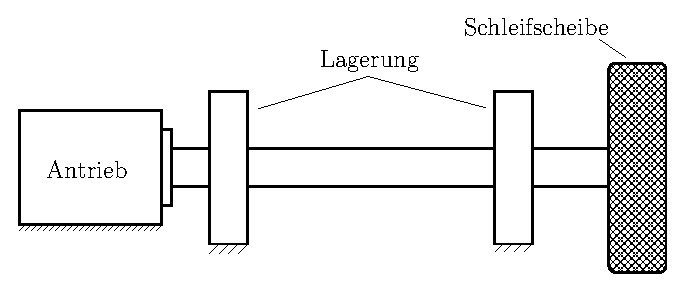
\includegraphics{./images/schema}
  \caption[Welle: schematischer Aufbau]{Schematischer Aufbau}
  \label{fig:schema}
\end{figure}


\subsection{Ermitteln der statischen Größen}
\label{sec:ermitt-der-stat}

Der statische Freischnitt ist in Abb.~\ref{fig:freischnitt} dargestellt. Für die Kräfteberechnung reicht es, das Gleichgewicht in vertikaler Richtung sowie das Momentengleichgewicht zu betrachten. Dies wird in Gl.~\eqref{eq:1} bis Gl.~\eqref{eq:6} durchgeführt. Der Berechnung liegen die Axiome von \cite{newton} zugrunde.

\begin{figure}[bt]
  \centering
  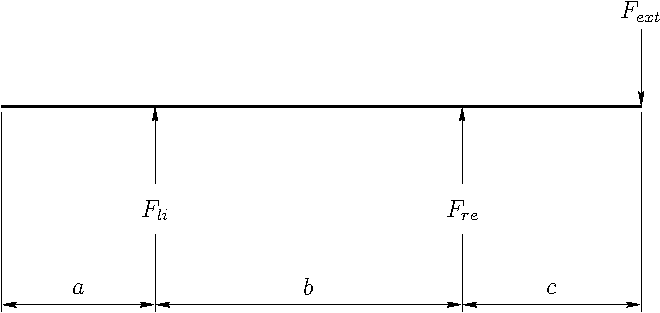
\includegraphics{./images/statik}
  \caption[Welle: statischer Freischnitt]{Freischnitt}
  \label{fig:freischnitt}
\end{figure}

Summe aller vertikalen Kräfte:
\begin{equation}
  \label{eq:1}
  \sum\limits_{i} F_{i}^{vert} = 0
\end{equation}
\begin{equation}
  \label{eq:2}
  -F_{li} - F_{re} + F_{ext} = 0
\end{equation}

Summe aller Momente:
\begin{equation}
  \label{eq:3}
  \sum\limits_{i} M_{i} = 0
\end{equation}
\begin{equation}
  \label{eq:4}
  -F_{re}b + F_{ext}(b+c) = 0
\end{equation}

Aus Gl.~\eqref{eq:4} folgt
\begin{equation}
  \label{eq:5}
  F_{re} = \frac{b+c}{b} F_{ext} 
\end{equation}

Diesen Ausdruck für $F_{re}$ in Gl.~\eqref{eq:2} eingesetzt liefert
\begin{equation}
  \label{eq:6}
  F_{li} = -\frac{c}{b} F_{ext} 
\end{equation}

Die gemessenen Werte an der Welle werden in Tabelle \ref{tab:wertewelle} (Seite~\pageref{tab:wertewelle}) verdeutlicht. Diese in die Gleichungen für $F_{li}$ und $F_{re}$ eingesetzt liefern die Zahlenwerte der gesuchten Größen.

\begin{table}[bt]
  \centering
  \begin{tabular}{|l|c|r|l|}
\hline
externe Kraft & $F_{ext}$ & 5.00 & $\unit{kN}$ \\
\hline
Abstand       & $a$       & 40    & \unit{mm}   \\
\hline
Abstand       & $b$       & 80    & \unit{mm}   \\
\hline
Abstand       & $c$       & 50    & \unit{mm}   \\
\hline
  \end{tabular}
  \caption{Gemessen Werte an der Welle}
  \label{tab:wertewelle}
\end{table}

\begin{equation}
  \label{eq:9}
  \begin{aligned}
    F_{li} & = -\frac{50}{80}\cdot 5.00 \\
           & = \unit[3.125]{kN}    
  \end{aligned}
\end{equation}

\begin{equation}
  \label{eq:10}
  \begin{aligned}
    F_{re} & = \frac{80 + 50}{50} \cdot 5.00 \\
           & = \unit[13.00]{kN}    
  \end{aligned}
\end{equation}

\section{Weitere Vorgangsweise}
\label{sec:weit-vorg}

In weiterer Folge wird das dynamische Verhalten der Welle mithilfe einer Computersimulation untersucht. Der nächste Projektbericht soll darüber Aufschluss geben.


%%%
%%% end main document
%%%
%%%%%%%%%%%%%%%%%%%%%%%%%%%%%%%%%%%%%%%%%%%%%%%%%%%%%%%%%%%%%%%%%%%%%%%%%%%%%%%%

 \appendix  %% include it, if something (bibliography, index, ...) follows below


% \lstlistoflistings
% \addcontentsline{toc}{section}{Code-Ausschnitte}

% \listoffigures
% \addcontentsline{toc}{section}{Abbildungsverzeichnis}

 

%%%%%%%%%%%%%%%%%%%%%%%%%%%%%%%%%%%%%%%%%%%%%%%%%%%%%%%%%%%%%%%%%%%%%%%%%%%%%%%%
%%%
%%% bibliography
%%%
%%% available styles: abbrv, acm, alpha, apalike, ieeetr, plain, siam, unsrt
%%%
 \bibliographystyle{plain}

%%% name of the bibliography file
 \bibliography{projekt.bib}


\end{document}
%%% }}}
%%% END OF FILE
%%%%%%%%%%%%%%%%%%%%%%%%%%%%%%%%%%%%%%%%%%%%%%%%%%%%%%%%%%%%%%%%%%%%%%%%%%%%%%%%
%% Local Variables:
%% mode: outline-minor
%% OPToutline-regexp: "%% .*"
%% OPTeval: (hide-body)
%% emerge-set-combine-versions-template: "%a\n%b\n"
%% End:
%% vim:foldmethod=marker
